\documentclass[english,notitlepage]{revtex4-1}  % defines the basic parameters of the document
%For preview: skriv i terminal: latexmk -pdf -pvc filnavn



% if you want a single-column, remove reprint

% allows special characters (including æøå)
\usepackage[utf8]{inputenc}
\usepackage[english]{babel}


\usepackage{physics,amssymb}  % mathematical symbols (physics imports amsmath)
\include{amsmath}
\usepackage{graphicx}         % include graphics such as plots
\usepackage{xcolor}           % set colors
\usepackage{hyperref}         % automagic cross-referencing (this is GODLIKE)
\usepackage{subcaption}
\usepackage{listings}         % display code
\usepackage{float}
\usepackage{enumitem}
%\usepackage[section]{placeins}
\usepackage{algorithm}
\usepackage[noend]{algpseudocode}
\usepackage{tikz}
\usetikzlibrary{quantikz}

\hypersetup{
    colorlinks,
    linkcolor={red!50!black},
    citecolor={blue!50!black},
    urlcolor={blue!80!black}}



\begin{document}

\title{Project 2}
\author{Alessio Canclini, Filip von der Lippe}
\date{\today}
\noaffiliation                            % ignore this, but keep it.


\maketitle

\textit{Github repository: \url{https://github.com/Fslippe/FYS4150/tree/main/project2}}
\\
\\
\section*{Introduction}
The main purpose og this project is to familiarize ourselves with the topics
of equation scaling, code testing and numerical solutions to eigenvalue problems. 
The eigenvalue problem we will be workning with is a special case of a 
one-dimensional buckling beam. \\
In problem 1 we will show how our initial second order differential equation
is scaled. Problems 2 through 4 focus on writing and testing the Jacobi roration algorithm we 
will be using to solve our eigenvalue problem. These do not appear in the report, 
but can be found in the Github repository linked above. In problem 5 we look at the 
algorithms scaling behavior, specifically how the the number of similarity transformations 
is related to the size $N$ of the input matrix. Finally in problem 6 we use the constructed code 
to solve our eigenvalue problem and make a plot of the three eigenvectors corresponding to the 
three lowest eigenvalues, visualizing the solutions to the differential equation for our buckling beam. \\
\\
\\


We are working with:
\begin{itemize}
    \item A horizontal beam of length $L$.

    \item We let $u(x)$ be the vertical displacement of the beam at horizontal position $x$, with $x \in [0,L]$.

    \item A force $F$ is applied at the endpoint $(x = L)$, directed into the beam, i.e. towards $x = 0$.

    \item The beam is fastened with pin endpoints, meaning that $u(0) = 0$ and $u(L) = 0$, but the endpoints are allowed to rotate $(u'(x) \neq 0)$.
\end{itemize}
Second order differential equation describing our buckling beam situation:
\begin{align}
    \gamma \frac{d^2u(x)}{dx^2} = - F u(x)
    \label{eq:diff}
\end{align}
Troughout this project we will be working with the scaled equation:
\begin{align}
    \frac{d^2u(\hat{x})}{d \hat{x}^2} = - \lambda u(\hat{x})
    \label{eq:scaled}
\end{align}
Where $\hat{x} \equiv x / L$ is a dimensionless variable, $\hat{x} \in [0,1]$ and $\lambda = \frac{FL^2}{\gamma}$.

\section*{Problem 1}
Using the defenintion $\hat{x} \equiv x / L$ to show that Eq. \ref*{eq:diff} can be written as Eq. \ref*{eq:scaled}.
\begin{align*}
    \gamma \frac{d^2u(x)}{dx^2} &= - F u(x)
\end{align*}
Dividing both sides by $\gamma$.
\begin{align*}
    \frac{d^2u(x)}{dx^2} &= - \frac{F}{\gamma} u(x)
\end{align*}
Multiplying both sides by $L^2$.
\begin{align*}
    \frac{d^2u(x)L^2}{dx^2} &= - \frac{FL^2}{\gamma} u(x) \\
    \frac{d^2u(x)}{d\frac{x^2}{L^2}} &= - \frac{FL^2}{\gamma} u(x)
\end{align*}
Using that $\hat{x} \equiv x / L$ so that $\hat{x}^2 \equiv x^2 / L^2$.
\begin{align*}
    \frac{d^2u(x)}{d\hat{x}} &= - \frac{FL^2}{\gamma} u(x)
\end{align*}
We also know that $x = \hat{x}L$, so $u(x) = u(\hat{x}L) = u(\hat{x}) + u(L) = u(\hat{x})$. Since $u(L) = 0$. Finally, using $\lambda = \frac{FL^2}{\gamma}$ gives us the dimensionless Eq. \ref*{eq:scaled}:
\begin{align*}
    \frac{d^2u(\hat{x})}{d\hat{x}} &= - \lambda u(\hat{x})
\end{align*}

\section*{Problem 5}
We will now look at how many similarity transformations we need 
before we reach a result where all non-diagonal matrix elements 
are close to zero. \\

Running our program for different choices of $N$
gives us the following scaling data in figure \ref{fig:N_iter_log_both}.
We obeserve that the number of required transformations $T$ are 
square proportional to the matrix size $N$. So $T = N^2$. \\

In figure \ref{fig:N_iter_log_both} we see that our program shows the close to
the same scaling behavior for both tridiagonal and dense matrixes. 
This is as expected, since our tridiagonal matrix is is 
no longer tridiagonal after the first jacobi rotation of our algorithm. 
Therfore the tridiagonal matrix is treated just like a dens matrix after a few
rotations in this case.

\begin{figure}[H]
    \centering
    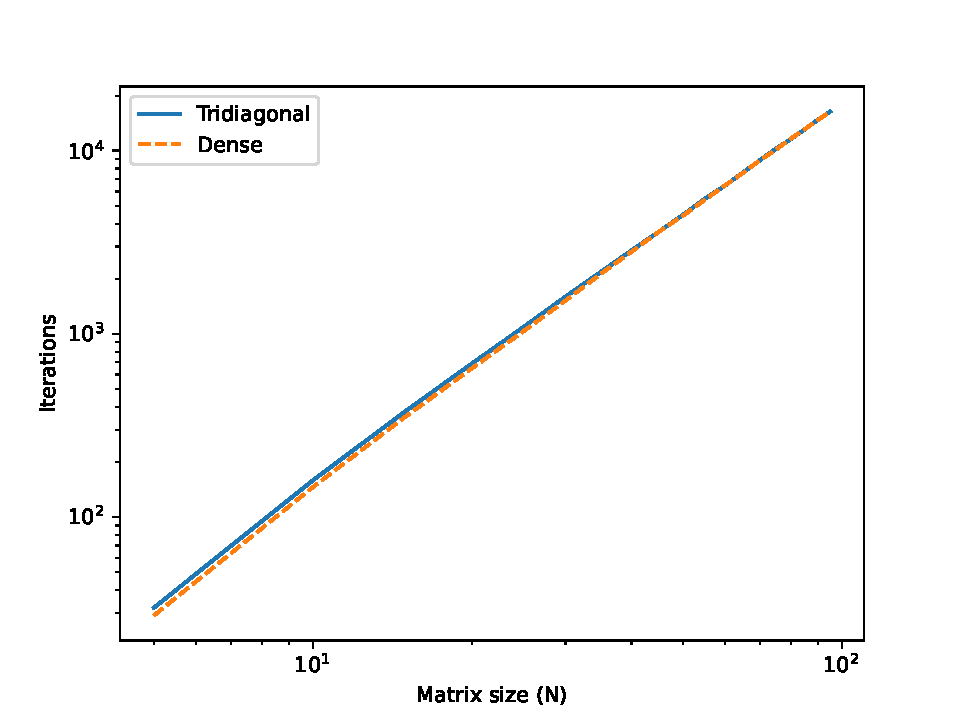
\includegraphics[width=1.\textwidth]{../figures/N_iter_log_both.pdf}
    \caption{Transformation scaling data for a matrixes on a Log scale.}
    \label{fig:N_iter_log_both}
\end{figure}


\newpage
\section*{Problem 6}
\begin{enumerate}[label= \alph*)]
    \item 
    Solving the equation $\bf{A} \vec{v} = \lambda \vec{v}$ for a discretization 
    of $\hat{x}$ with steps $n = 10$ steps gives us the three eigenvectors in figure
    \ref{fig:eigvec_10}

    \begin{figure}[H]
        \centering
        \begin{subfigure}{.45 \textwidth}
        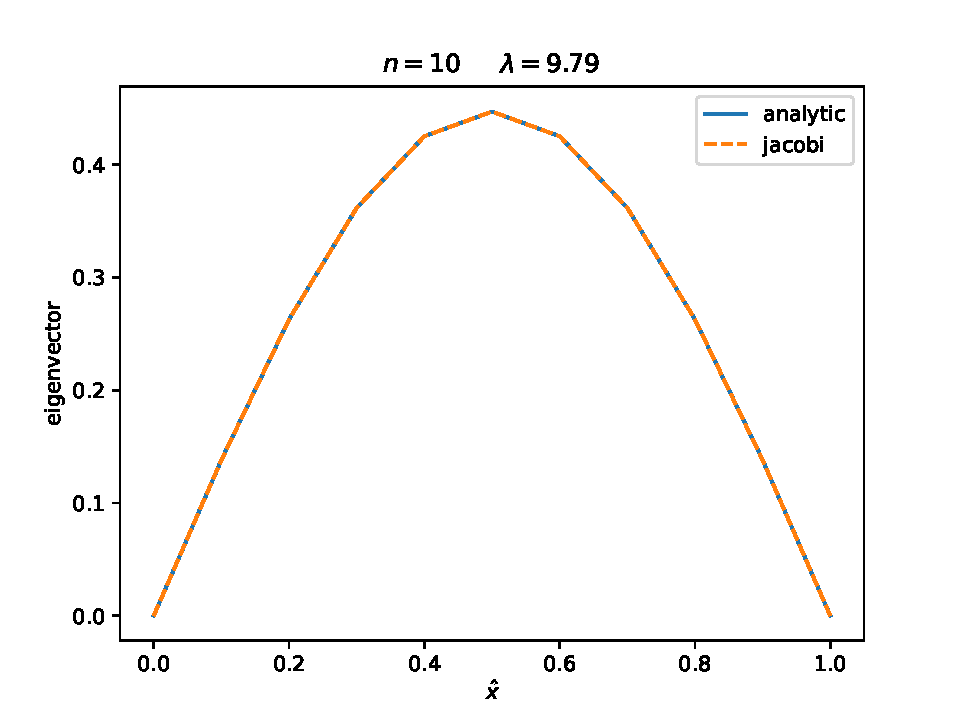
\includegraphics[width=1.1\textwidth]{../figures/eigvec_10_0.pdf}
        \caption{}
        \label{fig:eigvec_10_0}
    \end{subfigure}
    \begin{subfigure}{.45 \textwidth}
        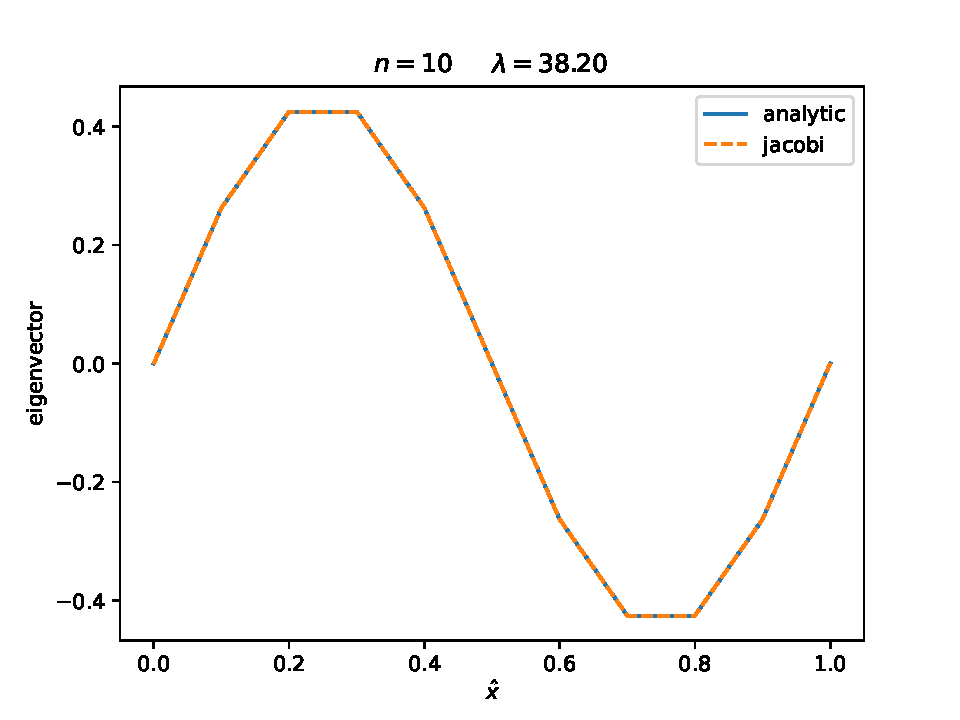
\includegraphics[width=1.1\textwidth]{../figures/eigvec_10_1.pdf}
        \caption{}
        \label{fig:eigvec_10_1}
    \end{subfigure}
    \begin{subfigure}{.45 \textwidth}
        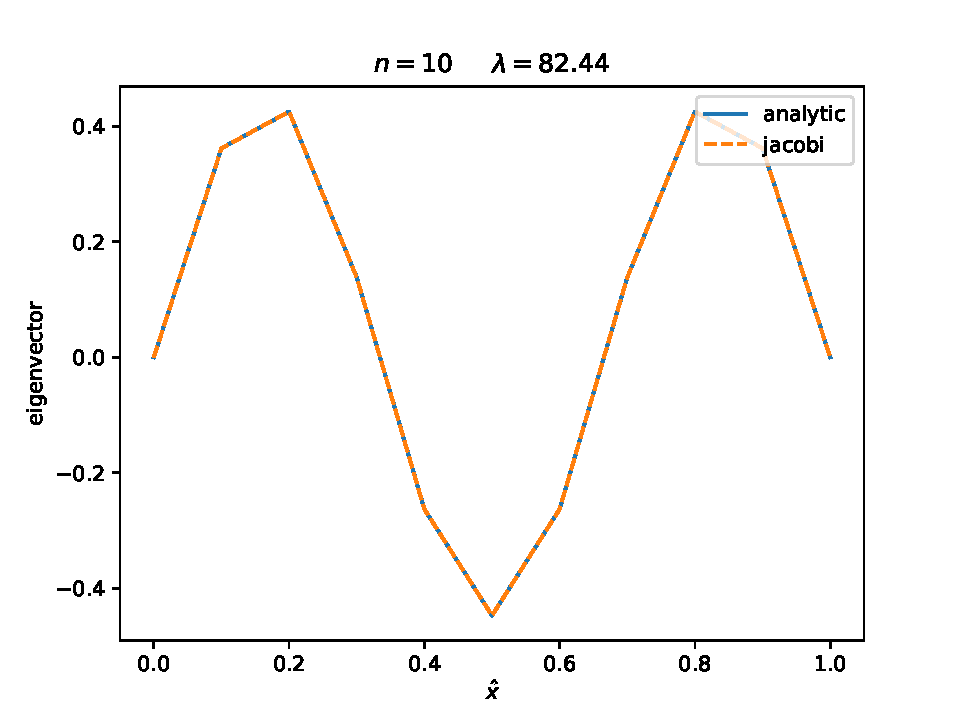
\includegraphics[width=1.1\textwidth]{../figures/eigvec_10_2.pdf}
        \caption{}
        \label{fig:eigvec_10_2}
    \end{subfigure}
    \caption{Eigenvectors corresponding to the three lowest eigenvalues for $n=10$. Shows the vector $v_i$ elements against the corresponding positions
}
    \label{fig:eigvec_10}
    \end{figure}
\newpage
    \item 
    Figure \ref{fig:eigvec_100} shows the same plots for discretization of with $n = 100$ steps.
    

    \begin{figure}[H]
        \centering
        \begin{subfigure}{.45 \textwidth}
        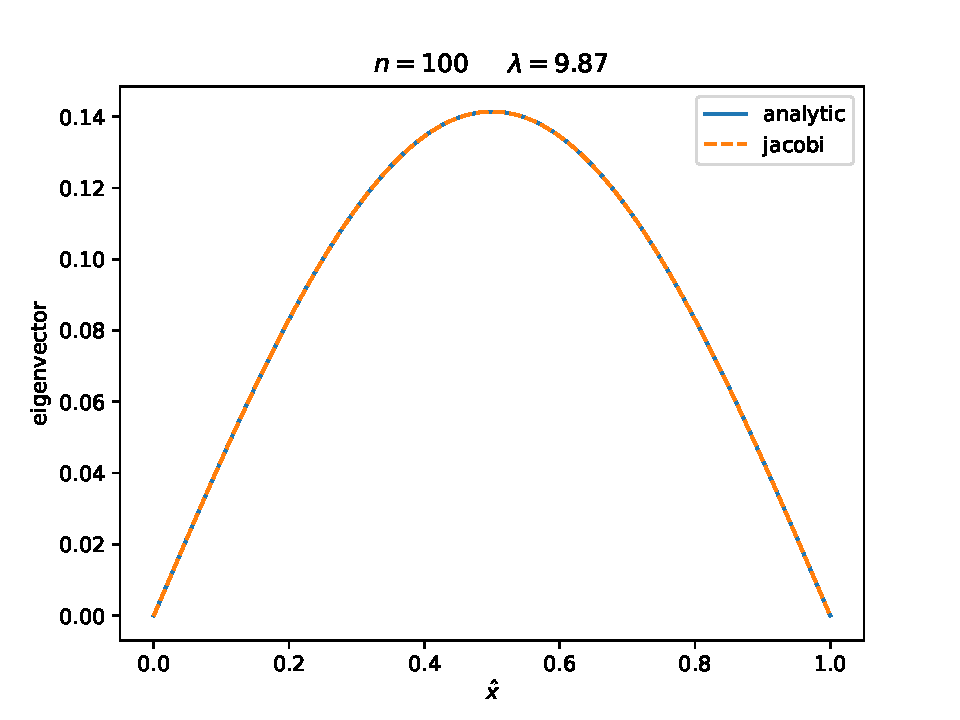
\includegraphics[width=1.1\textwidth]{../figures/eigvec_100_0.pdf}
        \caption{}
        \label{fig:eigvec_100_0}
    \end{subfigure}
    \begin{subfigure}{.45 \textwidth}
        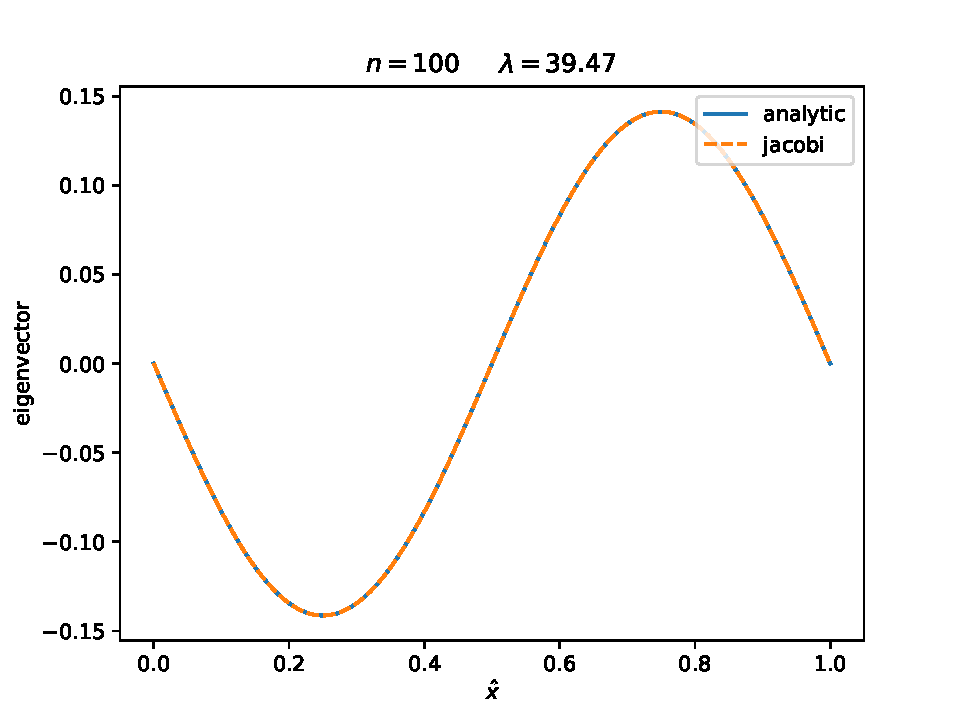
\includegraphics[width=1.1\textwidth]{../figures/eigvec_100_1.pdf}
        \caption{}
        \label{fig:eigvec_100_1}
    \end{subfigure}
    \begin{subfigure}{.45 \textwidth}
        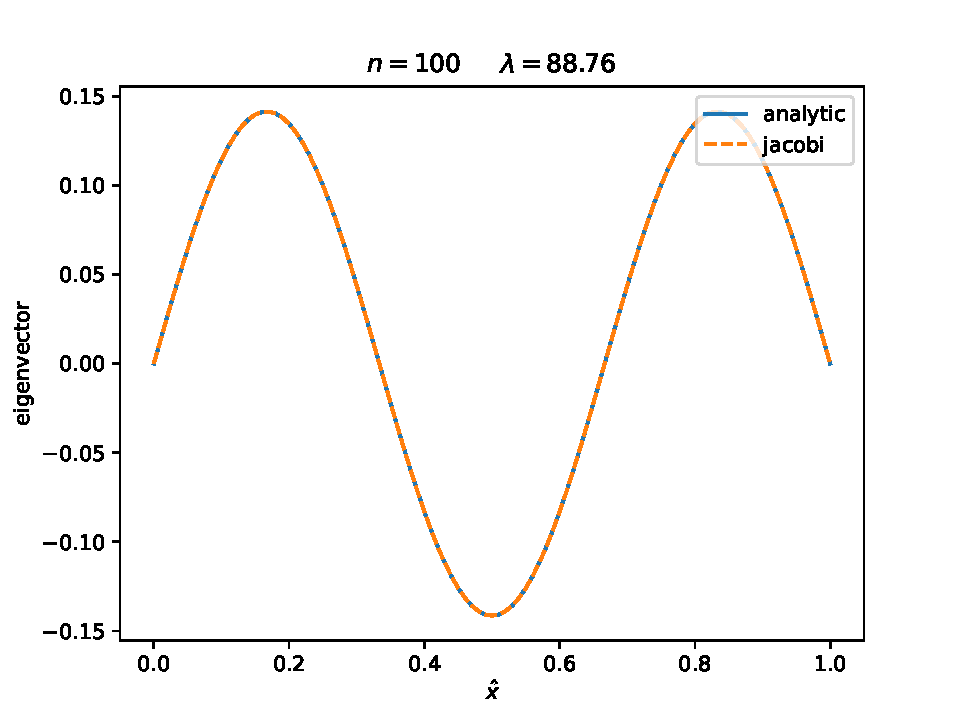
\includegraphics[width=1.1\textwidth]{../figures/eigvec_100_2.pdf}
        \caption{}
        \label{fig:eigvec_100_2}
    \end{subfigure}
    \caption{Eigenvectors corresponding to the three lowest eigenvalues for $n=100$.}
    \label{fig:eigvec_100}
    \end{figure}

\end{enumerate}

\end{document}
